For infected individuals, the time at risk was taken to be the time from start of follow-up to infection. For those who did not get infected the time at risk was take to be the time from start of follow-up to end of follow-up.

The model was

\begin{align*}
\begin{gathered}
h(t) = h_0\text{exp}(\beta_T X_{\text{logtitre}})
\end{gathered}
\end{align*}

where $h$ is the hazard function and $X_{\text{logtitre}}$ is the post-vaccination titre measurement on the log scale. The resulting protection curves (relative to the titre of 5) are in Figure \ref{fig:kiddyvaxmain-cox}. Although the point estimates are similar to those recovered from the model; however standard errors are inflated.

\begin{figure}[htp]
	\centering
	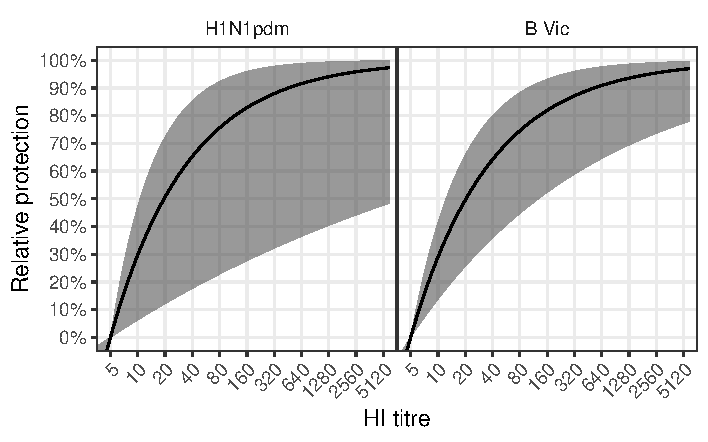
\includegraphics[width=0.8\textwidth]{../fit-cox-plot/kiddyvaxmain.pdf}
	\caption{
	Fitted relative-to-5 protection curves and confidence intervals from the Cox proportional hazards model fit to H1N1pdm and H3N2 subsets of kiddyvax data (shown in Figure \ref{fig:kiddyvax-main-titre}) with no accounting of censored titres (observations of 5 (below detectable) were unchanged, all other observations were moved to the midpoints of the corresponding censored intervals on a log scale). The solid line is the point estimates. The shaded region is the 95\% confidence interval.
	}
	\label{fig:kiddyvaxmain-cox}
\end{figure}
